% Final IEEE report. Compile with LaTeX and BibTeX using refs.bib.
\documentclass[conference]{IEEEtran}
\usepackage[T1]{fontenc}
\usepackage{amsmath,amssymb,bm,booktabs,graphicx,tabularx,array}
\usepackage{tikz,pgfplots,pgfplotstable}
\pgfplotsset{compat=1.18}
\usepgfplotslibrary{groupplots}
\pgfplotsset{reportaxis/.style={width=0.94\columnwidth,height=0.67\columnwidth,
  label style={font=\fontsize{9}{11}\selectfont},
  tick label style={font=\fontsize{9}{10}\selectfont},
  legend style={font=\fontsize{9}{10}\selectfont,draw=none,fill=white},
  grid=major,grid style={black!12},mark size=1.3pt,clip=true}}
\usetikzlibrary{arrows.meta,positioning}
\usepackage{cite}
\usepackage[hidelinks]{hyperref}
\newcolumntype{Y}{>{\raggedright\arraybackslash}X}
\newcommand{\E}{\mathbb{E}}
\newcommand{\F}{\mathbf{F}}
\newcommand{\J}{\mathbf{J}}
\title{Identifiability-Guided Active Calibration for Semi-Supervised ISAC:\\Reproduction, Controlled Evaluation, and Label-Budget Experiments}
\author{\IEEEauthorblockN{Muneef Mohammed, Andrew Liang, and Mohammad Al-Shammeri}
\IEEEauthorblockA{CISC 867: Deep Learning, Queen's University\\Final report draft, November 16, 2026}\\
\textbf{GitHub Repository:} \url{https://github.com/muneefo/DL_FINAL_REPORT}}
\pgfplotstableread{
x y
1.0000000000 0.17507789080
200.00000000 0.15504450710
400.00000000 0.14268434369
600.00000000 0.13500948631
700.00000000 0.13248621262
800.00000000 0.12971113825
1000.0000000 0.12526719288
1500.0000000 0.11073759550
2000.0000000 0.095768142221
2500.0000000 0.088214919857
3000.0000000 0.083922440324
3500.0000000 0.079962233666
5000.0000000 0.071361218199
6500.0000000 0.069867067691
8000.0000000 0.067264737950
10000.000000 0.064530990492
}\MeasuredSL
\pgfplotstableread{
x y
1.0000000000 6.3385435869
200.00000000 4.4637768709
400.00000000 3.9751347415
600.00000000 3.6163486416
700.00000000 3.4324377805
800.00000000 3.5075648916
1000.0000000 3.4251652301
1500.0000000 3.2136033350
2000.0000000 2.8417235154
2500.0000000 2.6845968697
3000.0000000 2.5910281541
3500.0000000 2.5056671162
5000.0000000 2.5142228747
6500.0000000 2.6963097484
8000.0000000 2.3051556319
10000.000000 2.4727785845
}\LocalizationSL
\pgfplotstableread{
x y
1.0000000000 0.17407412099
200.00000000 0.11464578129
400.00000000 0.10151205178
600.00000000 0.098562230941
700.00000000 0.097685180771
800.00000000 0.097635256739
1000.0000000 0.097273540598
1500.0000000 0.096235727474
2000.0000000 0.097212915540
2500.0000000 0.097087611592
3000.0000000 0.096904207599
3500.0000000 0.096394516723
5000.0000000 0.096611938174
6500.0000000 0.097370369431
8000.0000000 0.096747907310
10000.000000 0.096671070705
}\MeasuredUL
\pgfplotstableread{
x y
1.0000000000 6.3992178674
200.00000000 3.3931195552
400.00000000 3.1809534175
600.00000000 3.1345822429
700.00000000 3.2499497820
800.00000000 3.1366535778
1000.0000000 3.1839184453
1500.0000000 3.2561678008
2000.0000000 3.2652108481
2500.0000000 3.1864110682
3000.0000000 3.1233621984
3500.0000000 3.2399125217
5000.0000000 3.0590971539
6500.0000000 3.2684649556
8000.0000000 3.1091751237
10000.000000 3.2709583416
}\LocalizationUL
\pgfplotstableread{
x y
100.00000000 0.17494529328
85000.000000 0.17494529328
}\BaselineDetection
\pgfplotstableread{
x y
100.00000000 6.4303271028
85000.000000 6.4303271028
}\BaselineLocalization
\pgfplotstableread{
x y
0.99999995831 0.17425832177
199.98159649 0.15607121472
399.99958368 0.14513581557
599.98536458 0.13995427452
699.92539460 0.13707166381
799.99911788 0.13438161727
999.99983325 0.12949572684
1499.9654728 0.11329846085
1999.8164651 0.099613544814
2499.9642509 0.086316989195
2999.9262581 0.081208084973
3499.6280648 0.078100180997
4999.9256914 0.070535165074
6499.5728958 0.068427403990
7999.9891778 0.067864681146
10000.000834 0.066211963474
12499.831407 0.064823732343
14999.650977 0.063498986146
19998.159649 0.062570561498
24999.623750 0.059171361694
29999.285091 0.058953349120
34996.254388 0.058393314009
39999.938359 0.059351609918
44999.227432 0.058730029123
49999.244408 0.056831128712
54998.104821 0.056280585722
59998.506445 0.057277666639
64995.777728 0.056697150323
69992.504447 0.056342097384
74986.836533 0.056502000490
79999.871769 0.056926492202
84997.134142 0.055847724613
}\PaperSL
\pgfplotstableread{
x y
0.99999995831 0.17486551128
199.98159649 0.14369488446
399.99958368 0.12243777388
599.98536458 0.11080421055
699.92539460 0.10644535396
799.99911788 0.10464783893
999.99983325 0.10116514929
1499.9654728 0.10000993441
1999.8164651 0.096582258240
2499.9642509 0.096840518767
2999.9262581 0.096601922920
3499.6280648 0.095957241229
4999.9256914 0.098163767998
6499.5728958 0.097742236194
7999.9891778 0.096797310906
10000.000834 0.097182915544
12499.831407 0.098436691979
14999.650977 0.098213644158
19998.159649 0.098226198253
24999.623750 0.097065982145
29999.285091 0.098290329605
34996.254388 0.098004137068
39999.938359 0.095904371139
44999.227432 0.095698096132
49999.244408 0.095342873085
54998.104821 0.095946898560
59998.506445 0.095255776925
64995.777728 0.097985561090
69992.504447 0.094717822052
74986.836533 0.095946082034
79999.871769 0.096097479655
84997.134142 0.094739664135
}\PaperUL
\pgfplotstableread{
x y
0.0076863900758 0.99009811387
0.0077086621895 0.98995782337
0.0077242054977 0.98954745315
0.0077396128327 0.61954003726
0.0084185739979 0.42205103217
0.0095474673435 0.32247048552
0.011384456418 0.26575644828
0.011439833790 0.26415341991
0.014712984674 0.22454690783
0.022927077487 0.19505557355
0.53176903725 0.17473538653
0.53189104795 0.17425753661
0.53197187185 0.17401886337
}\BaselineJointDetection
\pgfplotstableread{
x y
0.0076863900758 83.641956194
0.0077098337933 82.888986113
0.0077127311379 81.200685330
0.0077396128327 12.105791492
0.0084185739979 9.0644957851
0.0090239224955 8.7893919561
0.0095474673435 7.8961670363
0.0096956156194 7.7095016331
0.011384456418 7.3607649318
0.011439833790 7.3397387348
0.012285390869 7.2794242102
0.012699984014 7.2656033054
0.014452301897 7.1511913905
0.014712984674 6.7246179935
0.015981797129 6.6276494473
0.022927077487 6.3053346256
0.53176903725 6.2905616580
}\BaselineJointLocalization
\pgfplotstableread{
x y
0.0013143327087 0.98845056373
0.0013167252764 0.98844335673
0.0013274055673 0.98835190163
0.0015008789487 0.35644595396
0.0015218944754 0.34892585823
0.0015454362147 0.34739939162
0.0017941829283 0.20175194343
0.0018172070850 0.19891191024
0.0018440950662 0.19796544737
0.0022284765728 0.14159251388
0.0022394564003 0.14029318434
0.0022749870550 0.13812808431
0.0029564616270 0.10921852200
0.0029573601205 0.10736917145
0.0030087435152 0.10687960359
0.0044180955738 0.088205947049
0.0044213901274 0.087319909322
0.0045514386147 0.086945174678
0.0085955439135 0.074825785238
0.0086771482602 0.073637638528
0.36525952816 0.064800366918
0.36557662487 0.064672812987
0.36565452814 0.064542958998
0.36567062140 0.064164922374
0.36570385098 0.063975410551
}\SLJointDetection
\pgfplotstableread{
x y
0.0013143327087 77.168218736
0.0013173340121 76.074270626
0.0015008789487 6.4373557124
0.0015166015364 6.2529963293
0.0015218944754 6.1886138686
0.0015454362147 6.1081438051
0.0017941829283 4.3422460602
0.0018440950662 4.3188970877
0.0022284765728 3.5874655862
0.0022749870550 3.5124624496
0.0023489224259 3.4183258650
0.0029564616270 3.0704935551
0.0031101789791 3.0337257414
0.0044180955738 2.8376077361
0.0044213901274 2.8079354987
0.0044984114356 2.7650552573
0.0047349054366 2.7526694432
0.0047718910500 2.7492943588
0.0085955439135 2.4317064875
0.0091615822166 2.4143979924
0.36525952816 2.3645288402
0.36527442932 2.1765351552
}\SLJointLocalization
\pgfplotstableread{
x y
0.0012548242230 0.98946321022
0.0012571223779 0.98929936604
0.0014527473832 0.45708966247
0.0017409733264 0.28061536177
0.0021515430417 0.20275383472
0.0028301042039 0.15888418649
0.0041575455107 0.13109206730
0.0045411358587 0.13085518019
0.0080053219572 0.11077824836
0.29254966974 0.096647582471
}\ULJointDetection
\pgfplotstableread{
x y
0.0012548242230 80.238591966
0.0012558919843 79.875058004
0.0014527473832 8.1941923079
0.0014566276222 8.1610573443
0.0014670150122 7.9575359062
0.0017409733264 5.5322222650
0.0017534537474 5.4547103656
0.0021515430417 4.5947975846
0.0022339355201 4.5397470626
0.0028301042039 4.0595625444
0.0028756249230 3.9689244695
0.0029169823974 3.8493412485
0.0041575455107 3.7429198121
0.0043419334106 3.7002950512
0.0045213899575 3.6011858216
0.0045411358587 3.5694556757
0.0080053219572 3.2902795725
0.29254966974 3.2602963456
0.29267945886 3.1772317663
0.29286962748 3.1597989543
}\ULJointLocalization
\pgfplotstableread{
x y
0.0077368430587 0.98972412985
0.0077126764752 0.61816934388
0.0083559490523 0.42151862412
0.0095599969476 0.32259086642
0.011310930778 0.26373847176
0.014663143484 0.22452920241
0.023139236071 0.19506362712
0.53205247498 0.17410014200
}\PaperJointBaselineDetection
\pgfplotstableread{
x y
0.0012452990745 0.98840378379
0.0014416223812 0.30520292178
0.0017005140047 0.17367242642
0.0021198463596 0.12286602544
0.0027733378225 0.094218621893
0.0040520892756 0.077512846202
0.0077469985826 0.065027237607
0.38138556431 0.055787472512
}\PaperJointSLDetection
\pgfplotstableread{
x y
0.0077368430587 84.748235413
0.0077126764752 12.119433424
0.0083559490523 9.0398419543
0.0095599969476 7.8850279263
0.011310930778 6.9728769753
0.014663143484 6.9667522593
0.023139236071 6.4855689556
0.53205247498 6.4006765503
}\PaperJointBaselineLocalization
\pgfplotstableread{
x y
0.0012452990745 78.001732349
0.0014416223812 5.7565005460
0.0017005140047 3.9604247666
0.0021198463596 3.2583139359
0.0027733378225 2.6454958590
0.0040520892756 2.6115093698
0.0077469985826 2.4065731823
0.38138556431 2.1281011329
}\PaperJointSLLocalization

\pgfplotstableread{
x y err
10.00000000 0.3122448327 0.1025309974
15.00000000 0.2104635412 0.07617585500
20.00000000 0.1894636753 0.05930301002
25.00000000 0.1722859506 0.04189098907
30.00000000 0.1653193889 0.04389479078
35.00000000 0.1641369275 0.04012756697
40.00000000 0.1558305815 0.03191420292
45.00000000 0.1632943854 0.02762481615
50.00000000 0.1600610840 0.02234842916
55.00000000 0.1613780592 0.05616589450
60.00000000 0.1615954511 0.03719130286
}\Activeweak
\pgfplotstableread{
x y err
10.00000000 0.3127896877 0.1026792621
15.00000000 0.2123017356 0.07634208879
20.00000000 0.1825003914 0.06524937056
25.00000000 0.1735140467 0.04158791046
30.00000000 0.1656300271 0.04359893077
35.00000000 0.1635055140 0.03984801670
40.00000000 0.1556203562 0.03336547865
45.00000000 0.1651286368 0.02575233674
50.00000000 0.1582952471 0.01607672681
55.00000000 0.1594681790 0.04994512709
60.00000000 0.1555401861 0.02765027249
}\Activefull
\pgfplotstableread{
x y err
10.00000000 0.3127896877 0.1026792621
15.00000000 0.2132187011 0.07696721459
20.00000000 0.1843886210 0.07421795809
25.00000000 0.1962861222 0.06237323264
30.00000000 0.1953549053 0.05740854997
35.00000000 0.1937010196 0.05007012660
40.00000000 0.1879424410 0.04037968847
45.00000000 0.1944199244 0.03539616546
50.00000000 0.1906413914 0.03163933533
55.00000000 0.1886519180 0.04666919985
60.00000000 0.1977882045 0.03927101211
}\Activerandom
\pgfplotstableread{
x y
10.00000000 0.3127896877
15.00000000 0.2225
20.00000000 0.1951
25.00000000 0.1922
30.00000000 0.2059
35.00000000 0.2169
40.00000000 0.2059
45.00000000 0.2082
50.00000000 0.2070
55.00000000 0.2023
60.00000000 0.1947
}\Activemaxangle
\pgfplotstableread{
x y
10.00000000 0.3127896877
15.00000000 0.2208
20.00000000 0.2093
25.00000000 0.2010
30.00000000 0.1971
35.00000000 0.1950
40.00000000 0.1904
45.00000000 0.1890
50.00000000 0.1825
55.00000000 0.1871
60.00000000 0.1836
}\Activediversity
\pgfplotstableread{
x y
10.00000000 0.3127896877
15.00000000 0.2207
20.00000000 0.2080
25.00000000 0.2269
30.00000000 0.2472
35.00000000 0.2644
40.00000000 0.2852
45.00000000 0.3071
50.00000000 0.3133
55.00000000 0.3231
60.00000000 0.3305
}\Activeuncertainty
\pgfplotstableread{
x y
1 0.17507789
200 0.15504451
400 0.14268434
600 0.13500949
700 0.13248621
800 0.12971114
1000 0.12526719
1500 0.06906698
2000 0.05856147
2500 0.05888377
3000 0.05861301
3500 0.05853806
5000 0.05893117
6500 0.0578652
8000 0.05884106
10000 0.0584767761809
}\MeasuredSSL
\pgfplotstableread{
x y
1 6.33854359
200 4.46377687
400 3.97513474
600 3.61634864
700 3.43243778
800 3.50756489
1000 3.42516523
1500 2.62146822
2000 2.18627647
2500 2.21369283
3000 2.25104616
3500 2.2982563
5000 2.27709382
6500 2.08501045
8000 2.07218304
10000 2.1587240158
}\LocalizationSSL

\pgfplotstableread{
x y
1.0000684585 0.17425831784
199.96003182 0.1560712289
400.03046934 0.14513580866
599.98652481 0.13995426172
699.8950631 0.13707166692
799.90273398 0.13438163469
1000.0630346 0.12949572137
1499.9708332 0.10215977724
1999.6099811 0.095853186304
2500.1651226 0.089810765978
2999.9427786 0.086308130853
3499.5361484 0.082915504978
5000.2513341 0.074214348471
6499.4171004 0.068925816148
7999.0573812 0.062191840209
10000.818668 0.057659125226
12500.854466 0.057516243061
14999.732362 0.05863618545
19996.196441 0.058979718548
25001.745122 0.059177549683
29999.508149 0.058004476352
34994.965354 0.058725714056
40003.390483 0.059489248739
45001.753135 0.058875163383
50002.701132 0.057824751292
55001.165827 0.059572803825
59999.103147 0.058271466759
64994.415098 0.058843143828
69990.032019 0.058885329499
74980.585672 0.058326972269
80006.724474 0.059119484093
85000.484617 0.058836576665
}\PaperSSL
\pgfplotstableread{
x y
0.0012318691475 0.98967371399
0.001233486788 0.98958311781
0.0012340899814 0.98955304942
0.0012452689996 0.98926590382
0.0014232517774 0.31285859308
0.0016917059997 0.17997261245
0.002097895857 0.12791220026
0.0021166740186 0.12768985759
0.0027602521553 0.098355437027
0.0027900208282 0.098156018597
0.0040560718606 0.080622828567
0.0040906930678 0.079628878524
0.0077237302224 0.067771196723
0.0079146200834 0.067668892208
0.4841089444 0.058685121366
0.48426378899 0.058424217359
}\SSLJointDetection
\pgfplotstableread{
x y
0.001231862753 82.248237528
0.0012334803831 81.857596079
0.0012340835726 80.150683019
0.0014232441282 5.8263588416
0.0016916965362 4.1848201657
0.001724481986 4.1671053764
0.0017358088231 4.1131550966
0.0020978835474 3.372335654
0.0021166615748 3.2459124463
0.0022096964042 3.2152011162
0.0027602349965 2.9443090699
0.0027900034462 2.8983950131
0.0029491726093 2.8492375124
0.0029603087189 2.7945112847
0.0040560446619 2.57689226
0.007723672106 2.3497561744
0.48410275535 2.0792522814
}\SSLJointLocalization
\pgfplotstableread{
x y
0.0012390145134 0.98953801557
0.0014291065917 0.31330302432
0.0016860107104 0.18009352166
0.0021010028719 0.12726576381
0.0027510859099 0.098129103256
0.0040324997493 0.0807545947
0.0077432030399 0.067486405511
0.49233329151 0.058643071943
}\PaperSSLJointDetection
\pgfplotstableread{
x y
0.0012390080727 83.120060657
0.0014290989036 5.9353858619
0.001686001286 4.0799617957
0.00210099054 3.4927942663
0.0027510688197 2.7223276182
0.0040324727386 2.655613495
0.0077431447522 2.4020694327
0.49232698676 2.1390786957
}\PaperSSLJointLocalization

\pgfplotstableread{
x y
1 0.174329256552
200 0.158581451077
400 0.145245583811
600 0.138297629163
700 0.13610897302
800 0.133825393261
1000 0.12766464152
1500 0.115747228377
2000 0.104262963238
2500 0.0945734202309
3000 0.0867619178393
3500 0.0830976103947
5000 0.0739329838085
6500 0.0725167407609
8000 0.0717144274692
10000 0.0672030589529
12500 0.0652658611612
15000 0.0667651884562
20000 0.0602536363229
25000 0.0605066026674
30000 0.0615328765056
35000 0.0623472354463
40000 0.0635645537827
45000 0.061192689112
50000 0.0589194611366
55000 0.0591717653389
60000 0.0589788004701
65000 0.0581651819353
70000 0.0581484650836
75000 0.0583948237871
80000 0.0583260198726
81000 0.0583648329599
82000 0.0580645374989
83000 0.0576381756214
84000 0.0580441160123
84200 0.0577756646832
85000 0.0578086942427
}\FullDetectionSL
\pgfplotstableread{
x y
1 6.4301906263
200 4.41911639119
400 4.04939431868
600 3.87356279386
700 3.77274248778
800 3.57168067424
1000 3.31557635668
1500 3.14058715076
2000 3.12330490989
2500 2.83904107901
3000 2.83098806539
3500 2.54883480387
5000 2.66205721589
6500 2.4037617926
8000 2.43703209577
10000 2.29800762752
12500 2.2935429837
15000 2.52957618963
20000 2.29782778346
25000 2.16878521722
30000 2.297558163
35000 2.19729083929
40000 2.17621482147
45000 2.27363077388
50000 2.28520713026
55000 2.09578784267
60000 2.21607288667
65000 2.07337947182
70000 2.20534498122
75000 2.31355110715
80000 2.15597466912
81000 2.12792440268
82000 2.1446030932
83000 2.19747722381
84000 2.12369269092
84200 2.14214082958
85000 2.29433858324
}\FullLocalizationSL
\pgfplotstableread{
x y
1 0.173759174751
200 0.113501461334
400 0.101611380613
600 0.0987292686791
700 0.0976770348867
800 0.0971167609843
1000 0.0970451744589
1500 0.0969571786693
2000 0.096556433669
2500 0.0972129324886
3000 0.0966802109337
3500 0.0965849996486
5000 0.0971790212516
6500 0.0965283264385
8000 0.096868659792
10000 0.0960677561293
12500 0.0972357682114
15000 0.0968549032959
20000 0.097516289622
25000 0.0969778236162
30000 0.0967985808588
35000 0.0974008058306
40000 0.0983298567684
45000 0.0975486696315
50000 0.0968680747072
55000 0.0960507486322
60000 0.0970477193677
65000 0.0968469850132
70000 0.0969108172099
75000 0.0964624492593
80000 0.0963478741901
81000 0.0965805623295
82000 0.0967844816505
83000 0.0963623378645
84000 0.096464232194
84200 0.0971817536613
85000 0.0973715761076
}\FullDetectionUL
\pgfplotstableread{
x y
1 6.42512216081
200 3.46776674492
400 3.45962922798
600 3.24561421665
700 3.08663691058
800 3.46175731761
1000 3.1770870192
1500 3.17595758139
2000 3.2946073657
2500 3.17047868407
3000 3.14678423931
3500 3.22801110097
5000 3.14809965493
6500 3.23951769255
8000 3.16614912135
10000 3.24328439127
12500 3.12715709053
15000 3.27147007541
20000 3.28020031061
25000 3.09356200785
30000 3.25231257552
35000 3.33162395283
40000 3.35404866656
45000 3.21613170558
50000 3.15017438614
55000 3.34004681449
60000 3.18913891035
65000 3.12799584972
70000 3.27126824345
75000 3.25723264945
80000 3.19611665646
81000 3.30706793616
82000 3.1098845603
83000 3.27101417758
84000 3.25582814557
84200 3.22056238181
85000 3.30526530244
}\FullLocalizationUL
\pgfplotstableread{
x y
1 0.175077890802
200 0.155044507104
400 0.142684343689
600 0.135009486315
700 0.13248621262
800 0.129711138247
1000 0.125267192881
1500 0.0690669799103
2000 0.0585614670576
2500 0.0588837696518
3000 0.0586130111555
3500 0.0585380629017
5000 0.0589311702132
6500 0.0578652005548
8000 0.0588410589641
10000 0.0584767761809
12500 0.0588568660083
15000 0.0582811036751
20000 0.059004453198
25000 0.0584155984607
30000 0.0586944132969
35000 0.0585667034442
40000 0.058501171914
45000 0.0584784167223
50000 0.0584102104679
55000 0.0583188252577
60000 0.0585024742574
65000 0.0581213642645
70000 0.0586724896612
75000 0.0583796987649
80000 0.0585204719543
81000 0.0590697173901
82000 0.0588545243157
83000 0.0583048615943
84000 0.0588669360739
84200 0.0585508704939
85000 0.0584079892678
}\FullDetectionSSL
\pgfplotstableread{
x y
1 6.33854358694
200 4.46377687085
400 3.97513474153
600 3.61634864159
700 3.43243778054
800 3.50756489161
1000 3.42516523008
1500 2.62146822211
2000 2.18627647288
2500 2.21369282866
3000 2.25104615683
3500 2.29825629724
5000 2.27709382339
6500 2.08501045128
8000 2.07218303758
10000 2.1587240158
12500 2.32066267819
15000 2.27058988109
20000 2.20486917208
25000 2.23501119853
30000 2.11539106011
35000 2.23212158327
40000 2.07417866519
45000 2.1883244093
50000 2.46194899334
55000 2.17054065877
60000 2.17115173878
65000 2.21818763434
70000 2.16101221472
75000 2.15900647811
80000 2.26964557742
81000 2.22072532774
82000 2.40795481749
83000 2.30574767437
84000 2.18310292137
84200 2.18987477119
85000 2.18035482067
}\FullLocalizationSSL


\begin{document}\maketitle
\begin{abstract}Position labels can constrain hardware parameters that remain ambiguous in unlabeled integrated sensing and communication (ISAC) measurements. We reproduce sequential semi-supervised learning and evaluate identifiability-guided acquisition of target-position labels. At 85,000 total updates, archived SSL with 1,000 supervised updates reaches misdetection probability 0.05841 and conditional position RMSE 2.180 m under the reproduction protocol, compared with 0.05781 and 2.294 m for full supervision. We then correct evaluation leakage and shared-range test batches by independently calibrating thresholds, selecting beams on validation observations, and testing frozen operating points. A fresh seed-42 sweep gives test misdetection probabilities 0.1402, 0.1405, 0.1051 and 0.0894 for 100, 500, 1,000 and 5,000 supervised updates, respectively, with total updates fixed at 85,000. The 5,000-update model has detected-target position RMSE 1.649 m. Across 176 active-calibration training runs, controlled ablations and three independent array draws, information-based variants select identical labels in all 72 hardware-study comparisons. Reconstructed label-information gains are nearly proportional. Guided-versus-random hardware intervals include zero, and fixed-label training is competitive. Independent localization confirms that a small range-error tail dominates unconditional RMSE. The completed experiments support sparse-supervision training and document the acquisition mechanism's lack of demonstrated benefit under the tested model.\end{abstract}
\begin{IEEEkeywords}ISAC, model-based learning, semi-supervised learning, active calibration, reproducibility.\end{IEEEkeywords}
\section{Introduction}
Integrated sensing and communication (ISAC) shares radio signals and hardware between environmental sensing and data delivery. Both tasks depend on accurate array responses. Antenna-location errors distort transmit beams and received-signal models, degrading detection, localization, and communication. Differentiable model-based learning embeds trainable calibration parameters within a physical processing pipeline, enabling structured adaptation without replacing every component with a generic neural network~\cite{icc,multi}.

Mateos-Ramos \emph{et al.}~\cite{ssl} introduce an unsupervised sensing objective for a single-target ISAC system and train it sequentially: supervised learning (SL) on labeled target positions, followed by unsupervised learning (UL) on unlabeled measurements. We refer to this sequence as semi-supervised learning (SSL). In their setting, SSL approaches SL performance with 98.8\% fewer labeled training samples. Acquiring reference positions may still require external sensors or controlled calibration, which raises a complementary question: \emph{which} positions should be labeled?

This project investigates \emph{whether position labels selected to inform weak hardware-calibration directions improve learning relative to random acquisition under matched budgets}. Unknown target geometry and hardware parameters can affect measurements similarly, so unlabeled observations may leave some calibration directions weakly constrained, while selected position references provide complementary information. As in our proposal, we keep the hardware fixed and consider a single target. Local information analysis guides the design; it does not establish global identifiability.

The completed project makes four contributions.
\begin{enumerate}
\item We reproduce SL, UL and sequential SSL at 85,000 updates and preserve the published-protocol comparison alongside the completed supervised-budget sweep.
\item We implement independent null calibration, validation-based beam selection and held-out operating-point tests, and document two defects in the inherited evaluator.
\item We evaluate fixed-label, full-trace and noRC controls across optimization seeds, independent hardware draws and angular coverage, with paired uncertainty and acquisition diagnostics.
\item We report sensing-SNR transfer and independent per-scene localization errors, providing a reproducible account of successful reproduction and the acquisition extension's null results.
\end{enumerate}
\section{Related Work}
\emph{Model-based learning and ISAC calibration.} Model-based deep learning combines domain-specific signal models with trainable components. Shlezinger \emph{et al.}~\cite{mbdl} review strategies that incorporate mathematical structure into learning systems, including communication and estimation applications. This perspective motivates our differentiable calibration parameters and structured receiver, but does not determine which observations should receive supervision.

Mateos-Ramos \emph{et al.}~\cite{icc} embed trainable steering matrices in a model-driven ISAC transceiver with $K=16$ antennas and compare it with a neural network under antenna-spacing errors of standard deviation $\lambda/30$. Without complexity limits, the network (about 6.4 million real parameters) slightly outperforms the model-driven design (8,000 complex parameters). When both are restricted to a few thousand parameters (about 5,000 real versus 2,500 complex), the network degrades while the model-driven design stays close to its unrestricted performance and generalizes better to an unseen angular sector. The semi-supervised framework~\cite{ssl} that we reproduce uses $K=64$ antennas, an unsupervised loss that maximizes the peak of the angle--delay map, and SL followed by UL. Over 85,000 total updates, spending about 1.2\% of them on SL matches full SL, whereas performance degrades when the labeled fraction falls below about 1\%. We reproduce this framework and study how reference positions are chosen, distinguishing unique acquired labels from their repeated use during optimization.

Several studies extend impairment learning. The multi-target framework~\cite{multi} uses a differentiable orthogonal matching pursuit for up to five targets with $K=64$. Learning the 64 spacing parameters directly, rather than a $64\times720$ dictionary (46,080 complex parameters), approaches the detection performance of a baseline with known impairments at $P_{\rm fa}=10^{-2}$ and converges faster. Gain--phase calibration~\cite{gain} learns per-antenna complex gain errors of a 64-element array without labels ($10^4$ updates, batch 1,024), with sensing performance close to the known-impairment case. Physically parameterized differentiable MUSIC (multiple signal classification)~\cite{music} learns antenna-location and complex-gain errors with supervised or unsupervised losses and estimates direction of arrival more accurately than classical MUSIC. A later multi-target preprint~\cite{multiul} calibrates arrays without labels using coherent received signals and alternative sensing objectives. All of these methods learn from unlabeled or randomly labeled data; none decides which observations to label.

\emph{Calibration ambiguity and statistical acquisition.} Weiss and Friedlander~\cite{weiss} estimate sensor locations jointly with the directions of sources at unknown locations by maximum likelihood. Their formulation exposes the coupling between hardware and target parameters that our nuisance elimination accounts for, and global motions of the array that such data cannot observe---the analogue of the translation gauge we remove in~\eqref{eq:calib}. Cohn, Ghahramani, and Jordan~\cite{cohn} derive closed-form query criteria that minimize the expected variance of a learner (mixtures of Gaussians and locally weighted regression) rather than maximizing prediction uncertainty. Our calibration-specific hypothesis follows the same logic: some uncertain positions carry less information about shared hardware than observations sensitive to its weak directions.

\emph{Diversity, gradient, and information-based selection.} Core-set acquisition~\cite{coreset} casts batch selection as a $k$-center problem in a network's feature space and reports gains over random and uncertainty sampling on image classification benchmarks (CIFAR-10/100, Caltech-256, SVHN). Our estimated-angle diversity rule is a simpler, task-specific version. BADGE~\cite{badge} samples diverse, high-magnitude last-layer gradient embeddings by $k$-means++ seeding; transferring it to position regression would require replacing its hallucinated class labels. BAIT~\cite{bait} greedily minimizes $\operatorname{tr}((\sum_{x\in S}\mathbf I(x))^{-1}\mathbf I_U)$, a trace criterion on last-layer Fisher information, oversampling $2B$ candidates and pruning to $B$. It matches or outperforms BADGE, Core-set, confidence, and random sampling on MNIST, SVHN, CIFAR-10, and OpenML classification and on regression tasks; its authors prefer the trace to the log-determinant, which our D-optimal comparator uses. Information-based selection is therefore not our contribution. We study the incremental information a position label provides about shared calibration parameters after nuisance elimination, with emphasis on weak directions that labels can constrain.

Appendix Table~\ref{tab:related} summarizes the reviewed works. A fair evaluation requires random, diversity, uncertainty, and conventional information comparators, isolated tests of weak-direction targeting and batch updating, and sensing--communication performance at matched labeling and computational budgets.



\emph{Optimization and uncertainty.} Our differentiable implementation uses PyTorch~\cite{pytorch} and Adam~\cite{adam}, following the original code's learning-rate settings. These software and optimizer choices support the model-based pipeline rather than defining the acquisition criterion. For independent test frames we report Wilson intervals~\cite{wilson} for detection and false alarms. These conditional test-frame intervals answer a different question from the Student-$t$ intervals over optimization seeds or independent hardware draws reported for the acquisition experiments. Both are needed because additional test frames do not create additional trained models or hardware replicates.
\section{System and Implemented Learning Method}
\subsection{Signal model and trainable component}
The transceiver has $K=64$ antenna elements and $S=256$ orthogonal frequency-division multiplexing (OFDM) subcarriers. With $k_c=k-(K-1)/2$ and wavelength $\lambda=c/f_c$, its steering model is
\begin{equation}
 a_k(\theta;\mathbf d)=\exp[-j(2\pi/\lambda)k_c d_k\sin\theta].
 \label{eq:steer}
\end{equation}
Here $k=0,\ldots,K-1$, $c$ is propagation speed, and $j^2=-1$. Parameters $d_k$ induce element positions $k_cd_k$; they are not adjacent gaps. The true fixed vector is $\mathbf d^\star$, while the estimator learns $\widehat{\mathbf d}$, initialized to $(\lambda/2)\mathbf1$. In our code, $\widehat{\mathbf d}$ is the only parameter of a small module (\texttt{PertNet}). Learning occurs by backpropagation through the structured beamformer and receiver rather than through a multilayer predictor.

For a present target at angle $\theta$, range $R$, delay $\tau=2R/c$, and complex reflection gain $\alpha$,
\begin{equation}
 \mathbf Y=\frac{\alpha}{\sqrt S}\mathbf a(\theta;\mathbf d^\star)
 \mathbf a^T(\theta;\mathbf d^\star)\mathbf f
 [\mathbf x\odot\bm\rho(\tau)]^T+\mathbf W,
 \label{eq:obs}
\end{equation}
where $\rho_s(\tau)=e^{-j2\pi s\Delta_f\tau}$, $\mathbf x$ contains known quadrature phase-shift keying (QPSK) symbols, $\mathbf f$ is a unit-norm beam, $\odot$ is elementwise multiplication, and noise entries are independent $\mathcal{CN}(0,N_0)$. For absent targets, $\mathbf Y=\mathbf W$. The physical array remains fixed while its learned model changes.

Reciprocal filtering removes symbols, yielding $\widetilde{\mathbf Y}$. The receiver forms a sector-masked angle--delay map
\begin{equation}
 M_{uv}=\left|\mathbf a^H(\theta_u;\widehat{\mathbf d})
       \widetilde{\mathbf Y}\bm\rho^*(\tau_v)\right|,
\end{equation}
where $H$ and $*$ denote Hermitian transpose and conjugation. The maximum of $M$ selects a window; softmax weighting inside it gives differentiable angle and range estimates and the Cartesian position $\widehat{\mathbf p}=[\widehat R\cos\widehat\theta,\widehat R\sin\widehat\theta]^T$. Note that $\widehat{\mathbf d}$ enters only the angular steering vectors; the delay response $\bm\rho$ does not depend on it.
\begin{figure}[t]\centering
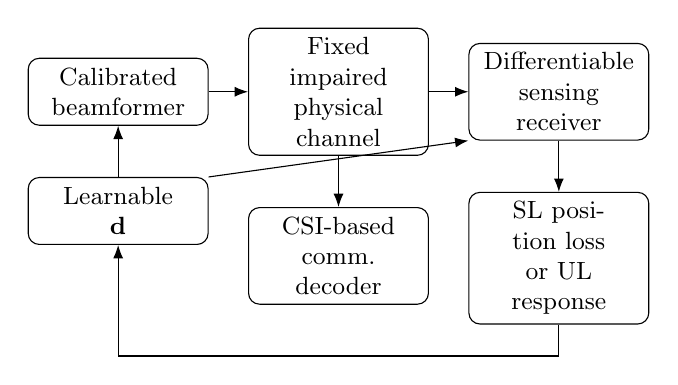
\begin{tikzpicture}[>=Latex,box/.style={draw,rounded corners,align=center,font=\small,text width=2.05cm,minimum height=.85cm},node distance=.5cm]
\node[box] (tx) {Calibrated\\beamformer};
\node[box,right=of tx] (ch) {Fixed impaired\\physical channel};
\node[box,right=of ch] (rx) {Differentiable\\sensing receiver};
\node[box,below=.65cm of tx] (d) {Learnable\\$\mathbf d$};
\node[box,below=.65cm of ch] (comm) {CSI-based\\comm. decoder};
\node[box,below=.65cm of rx] (loss) {SL position loss\\or UL response};
\draw[->] (tx)--(ch);\draw[->] (ch)--(rx);\draw[->] (ch)--(comm);
\draw[->] (rx)--(loss);\draw[->] (d)--(tx);
\draw[->] (d.north east)--(rx.south west);
\draw[->] (loss.south)--++(0,-.4)-|(d.south);
\end{tikzpicture}
\caption{Implemented differentiable pipeline. Gradients update the calibration model while the physical array remains fixed. Scene-label acquisition wraps the supervised and unsupervised updates.}
\label{fig:architecture}
\end{figure}
\subsection{Objectives and communication evaluation}
For minibatch size $B$, the position mean-squared error (MSE) minimized by SL and the peak objective maximized by UL are
\begin{align}
 L_{\rm SL}&=\frac{1}{2B}\sum_i\|\widehat{\mathbf p}_i-\mathbf p_i\|_2^2,\\
 U_{\rm UL}&=\frac1B\sum_i\max_{u,v}M^{(i)}_{uv}.
\end{align}
Both use the Adam optimizer~\cite{adam} in PyTorch~\cite{pytorch}. SL uses present targets. The original online UL randomizes target presence, whereas the pilot uses present-target pools. Labels used for diagnostic metrics never enter the UL objective.

For sensing and communication beams $\mathbf f_r,\mathbf f_c$, joint evaluation sweeps
\begin{equation}
 \mathbf f(\eta,\phi)=
 \frac{\sqrt\eta\mathbf f_r+\sqrt{1-\eta}e^{j\phi}\mathbf f_c}
 {\|\sqrt\eta\mathbf f_r+\sqrt{1-\eta}e^{j\phi}\mathbf f_c\|_2},
\end{equation}
where $\eta\in[0,1]$ controls allocation and $\phi$ is relative phase. The communication receiver uses the effective channel state information (CSI) and maximum-likelihood symbol decisions; imperfect CSI is not studied. The trade-off curves select operating points across beams; they are not a multiobjective training loss.

\subsection{Metrics and physical settings}
We use $K=64$, $S=256$, carrier frequency 60 GHz, subcarrier spacing 120 kHz, a 720-point angle grid, and a 200-point range grid over $[0,200]$ m. Communication uses QPSK, five normalized exponentially weighted taps and SNR 20 dB. Default sensing SNR is 15 dB. Training sector centres are uniform over $[-60,60]^\circ$ for reproduction and the online fraction sweep. Active experiments also use the narrow $[-10,10]^\circ$ centre support, with sector widths uniform over $[10,20]^\circ$.

Detection metrics are $P_{\rm md}=P(\widehat t=0\mid t=1)$ and $P_{\rm fa}=P(\widehat t=1\mid t=0)$, with nominal false-alarm target 0.01. Communication SER is the fraction of incorrectly decoded symbols. The detected-target position metric is
\begin{equation}
 \mathrm{RMSE}_{\mathrm{det}}=\sqrt{\E[\|\widehat{\mathbf p}-\mathbf p\|_2^2\mid t=1,\widehat t=1]}.
\end{equation}
Localization-only tests evaluate all present scenes and report unconditional position RMSE and median position error. Their conditioning and angular distribution differ from the joint detection test, so both protocols are specified with every table.
\section{Identifiability-Guided Acquisition}
\subsection{Implemented information and selection}
Normalize hardware as $\mathbf u=\mathbf d/(\lambda/2)$. Observation-specific nuisances are angle, normalized range, and the real and imaginary parts of the gain. Holding the transmitted beam fixed, the real-stacked mean of~\eqref{eq:obs} has Jacobian $\J$ and Fisher information
\begin{equation}
 \mathbf I=\frac{2}{N_0}\J^T\J.
\end{equation}
Schur elimination (Appendix~A) gives $\F_U$ when position is unknown and $\F_L$ when position is known but gain is not. The estimated label gain is $\Delta\F_i=\F_{L,i}-\F_{U,i}$. Because the mean in~\eqref{eq:obs} is linear in $\alpha$, $\Delta\F_i$ scales with $|\alpha_i|^2$. Before querying, we evaluate it at the current receiver positions and least-squares gain estimates. Hidden positions enter only the physical simulator, revealed-label SL, and diagnostics.

The code adds $12/w_i^2$ to the angle-information diagonal for sector width $w_i$. This inverse-variance precision is a soft approximation to a bounded uniform prior, not its exact Fisher information. Trace-scaled ridges stabilize nuisance solves.

Shifting all induced element positions changes a phase absorbable by the unknown gain. Its direction has entries proportional to $1/k_c$; these are finite for even $K=64$. Let $\mathbf Q$ span its orthogonal complement. The calibration metric is
\begin{equation}
 e_d=\left\|\mathbf Q^T
       \frac{\widehat{\mathbf d}-\mathbf d^\star}{\lambda/2}\right\|_2,
 \label{eq:calib}
\end{equation}
a dimensionless norm, not per-element RMSE. Weak selection uses eigenvectors $\mathbf V$ on this subspace with eigenvalues below $10^{-3}$ times the largest, retaining the weakest if none qualify, and scores
\begin{equation}
 s_i=\operatorname{tr}(\mathbf V^T\Delta\F_i\mathbf V).
 \label{eq:score}
\end{equation}
Greedy batch selection updates the information after each provisional choice (redundancy control). Current information is approximated from labeled scenes and sampled candidates, not the full pool, using plug-in receiver estimates. Fig.~\ref{fig:workflow} and Appendix~A summarize the loop.

\subsection{Pilot protocol and comparators}
A fixed scene stores geometry, reflection gain, presence, and sectors. Measurements are re-synthesized with the current beam and fresh symbols and noise whenever a scene is used. This is repeated interrogation of fixed scenes, not selection from immutable recordings, and assumes that scenes can be revisited while reference positions remain valid.

The pilot starts with 10 random labels and queries five per round until 60 labels are acquired. It performs 100 SL plus 100 UL updates initially and after each of the ten query rounds: 1,100 updates of each kind and 140,800 training scene exposures. SL samples acquired scenes with replacement; UL samples all training scenes without their labels. Up to 300 candidates are scored per round. Learning rates are ten times the reproduction values, with no scheduler.

The original comparator set contains six acquisition rules: weak projection~\eqref{eq:score}; D-optimal information, the largest increase in the log-determinant of the gauge-free information; random; the largest estimated $|\theta|$ (max.\ angle); farthest-angle diversity; and the largest position Cram\'er--Rao bound (uncertainty). The uncertainty rule treats hardware as known and gain as a nuisance; it is not an ensemble estimate. D-optimal changes both the projection and the scalar objective, so we treat it as a comparator rather than a projection-only ablation. We also evaluate noRC, a full-trace control retaining every gauge-free direction, and a fixed-label control retaining only the initial 10 labels through the same training schedule.

All rules share the fixed hardware and pools, seeds 0--4, update counts, and initial label indices. The corrected implementation restores CPU, CUDA and NumPy random states around scoring and validation. Scoring uses separately seeded measurements, and parameter histories store independent copies of every round. Mini-batch selection uses a private generator. These repairs were checked by replaying initial models and by an interrupted/resumed training smoke test.

\section{Experimental Protocols}\label{sec:protocols}
\subsection{Experiment cohorts and budgets}
Table~\ref{tab:settings-final} records the budgets used in each cohort. The archived reproduction uses the original fixed array and online random training examples. SL minimizes position MSE for all 85,000 updates. UL maximizes the receiver peak objective for all updates. Archived SSL uses 1,000 SL and 84,000 UL updates. The new online sweep fixes the total at 85,000 and runs seed 42 with 100, 500, 1,000 and 5,000 SL updates, followed by UL. A fresh seed-10 UL reference was completed first. Existing full-SL and UL archives are additional reference checkpoints.

The primary supervised-budget comparisons use seed 42. The extra seed-10 UL run is explicitly identified because its initialization and training stream differ. The archived SSL file does not save its training seed, and its early learning curve matches the original midterm trace. We therefore report its stored outputs without assigning the archive a newly verified seed. Every fresh sweep checkpoint records seed, update allocation, batch size, rates, hardware and elapsed time.

\subsection{Acquisition repetitions and controls}
The corrected fixed-array cohort runs ten variants across optimization seeds 0--4, totaling 50 runs. It includes weak, D-optimal, random, max-angle, diversity, uncertainty, full trace, fixed labels and weak/full noRC. All acquired labels are unique scene indices. The fixed-label control continues training on its original 10 labeled scenes through all 11 rounds, receiving the same 1,100 SL and 1,100 UL updates as an active rule.

The hardware study adds 126 runs from three independent array draws, two centre coverages, three optimization seeds and seven variants. The variants are weak, trace, D-optimal, random, fixed, weak noRC and full noRC. Hardware seeds 3101--3103 drive a private Gaussian draw with standard deviation $\lambda/25$, followed by the reference alternating-sort construction. Draws must have positive spacing parameters and strictly ordered induced element positions. All three proposed draws pass on their first attempt. Scene pools are shared across arrays within each coverage, keeping scene variation controlled.

Fixed-array intervals use five optimization seeds. Hardware-study intervals first average the three optimization seeds within each array, then use the three array means as independent replicates. Paired comparisons share the same seed or array. We use two-sided 95\% Student-$t$ intervals and retain their limited precision when only three arrays are available.

\subsection{Independent calibration, validation and test}
The inherited ISAC routine chooses thresholds on evaluated observations. It interpolates independently sorted PFA and PD/RMSE arrays, which discards the correspondence of individual operating points. In addition, the channel expands scalar angular limits to a batch but leaves scalar range limits unchanged. Consequently, its usual scalar-range call draws one range shared across a batch. We preserve those outputs for reproduction and implement a corrected evaluator for the completed tests below.

The corrected evaluator draws 10,000 absent-target calibration frames with seed 87001. With false-alarm target $\alpha_0=0.01$, the threshold is the order statistic at rank
\begin{equation}
 k=\lceil(n_0+1)(1-\alpha_0)\rceil,
\end{equation}
and a detection requires the metric to be strictly larger. If the rank exceeds the calibration size, the threshold is infinite. Under the additive-noise null, transmit-beam allocation does not affect the sensing observation, so calibration is shared across beams for a fixed receiver and sector. A replay test verifies that null-beam invariance.

Next, 10,000 validation frames at seed 88001 evaluate a $4\times4$ beam grid. Among beams with measured validation SER at most 1\%, we select the beam with lowest validation misdetection, breaking ties by SER and then grid index. If no beam is feasible, the output records this status. The selected beam and threshold are frozen before 20,000 test frames at seed 89001. Each frame receives an independently drawn range. We report measured test SER even when it exceeds the validation constraint, without changing the selected beam.

Wilson intervals quantify test-frame PMD and PFA uncertainty for each fixed operating point~\cite{wilson}. Symbol errors share a channel within each frame, so the saved SER standard error uses frame averages. Neither interval replaces repetition over trained models, hardware or scene pools. The original frontier protocol and this frozen-point test answer different evaluation questions, and the report labels their outputs accordingly.

\subsection{Generalization and independent localization}
Joint tests use sensing angles $[-40,-20]^\circ$ and communication angles $[30,50]^\circ$. For narrow active training, the sensing test is outside the training support. A separate central-sector evaluation uses $[-10,10]^\circ$ for sensing with the original communication sector. This central sector lies within narrow training support, although it is one fixed sector rather than the entire random-sector training distribution.

SNR transfer freezes model weights and changes test sensing SNR to 5, 10, 20 and 25 dB. The 15 dB sweep result completes the five-level curve. Threshold calibration and beam validation are rerun at each SNR, followed by independent testing. Communication SNR remains 20 dB. Thus the curves evaluate adaptation of the operating point at a changed sensing SNR, without retraining hardware parameters.

The localization-only evaluation draws 5,000 new present-target scenes with seed 93001 and fresh measurement noise with seed 94001. Sector centres follow each model's training coverage. It saves true and estimated angles/ranges, gain magnitudes and per-scene errors. This extends the original 500-scene validation metric with a separate scene pool and supports direct tail-error accounting.
\section{Results}\label{sec:results}
\subsection{Completed reproduction at 85,000 updates}
The original midterm checkpoint comparison reproduced SL and UL misdetection at 10,000 updates within 2.5\% and 0.5\% of approximate published-curve values. The completed full-budget archives appear in Table~\ref{tab:legacy-final}. Final sensing-only PMD is 0.05781 for SL, 0.09737 for UL and 0.05841 for archived SSL. The corresponding detected-target RMSEs are 2.294, 3.305 and 2.180 m. Figure~\ref{fig:learning} extends all measured learning curves to 85,000 updates.

\begin{figure}[t]\centering
\begin{tikzpicture}
\begin{groupplot}[reportaxis,width=0.88\columnwidth,group style={group size=1 by 2,vertical sep=0.8cm},
 xmode=log,xmin=100,xmax=85000,xtick={100,1000,10000,85000},
 xticklabels={$10^2$,$10^3$,$10^4$,$8.5\times10^4$}]
\nextgroupplot[ymin=0.04,ymax=0.19,ylabel={$P_{\rm md}$},
 legend style={at={(0.98,0.98)},anchor=north east},legend columns=2]
\addplot[blue,dashed] table {\PaperSL};\addlegendentry{Paper SL}
\addplot[blue,mark=*,mark size=1pt] table {\FullDetectionSL};\addlegendentry{Our SL}
\addplot[orange!85!black,dashed] table {\PaperUL};\addlegendentry{Paper UL}
\addplot[orange!85!black,mark=*,mark size=1pt] table {\FullDetectionUL};\addlegendentry{Our UL}
\addplot[red!75!black,mark=triangle*,mark size=1pt] table {\FullDetectionSSL};\addlegendentry{Our SSL}
\addplot[green!50!black,dashed] table {\PaperSSL};\addlegendentry{Paper SSL}
\nextgroupplot[ymin=0,ymax=7,ylabel={Position RMSE (m)},xlabel={Training updates},
 legend style={at={(0.98,0.84)},anchor=north east}]
\addplot[blue,mark=*,mark size=1pt] table {\FullLocalizationSL};\addlegendentry{Our SL}
\addplot[orange!85!black,mark=*,mark size=1pt] table {\FullLocalizationUL};\addlegendentry{Our UL}
\addplot[red!75!black,mark=triangle*,mark size=1pt] table {\FullLocalizationSSL};\addlegendentry{Our SSL}
\addplot[black!65,dashed] table {\BaselineLocalization};\addlegendentry{Untrained}
\end{groupplot}
\end{tikzpicture}
\caption{Completed SL, UL, and sequential SSL runs through 85,000 updates. Top: measured misdetection and approximate published SL/UL/SSL curves. Bottom: measured conditional position RMSE and the original untrained reference. SSL uses 1,000 SL followed by 84,000 UL updates. The measured curves use the full-run archives and the inherited sensing evaluation.}
\label{fig:learning}
\end{figure}

Archived SSL uses 98.8\% fewer supervised updates than full SL while reaching close detection and a slightly lower conditional RMSE in these stored runs. This is a supervised-update comparison. It does not measure the cost of repeatedly acquiring positions in the fixed-pool active experiment. The archive is one model per method, so the numerical closeness is reported descriptively.

\subsection{Main independent operating-point comparison}
Table~\ref{tab:main-final} evaluates the existing full-budget archives and two array controls with the corrected frozen-point test. The nominal control uses $\lambda/2$ in beam and receiver design. The known-array control uses the true fixed array without training. All models are tested at sensing SNR 15 dB, communication SNR 20 dB, and the same prescribed sectors. The selected beam can differ across models because selection uses each model's validation data.
\begin{table*}[t]\centering\small
\caption{Main independent-test results. PMD, PFA and SER are percentages. PMD intervals are Wilson intervals over test frames. RMSE is conditioned on detection.}\label{tab:main-final}
\setlength{\tabcolsep}{3pt}
\begin{tabular}{lrrrrr}\toprule
Model & PMD & 95\% CI & PFA & SER & RMSE (m)\\\midrule
Nominal array & 37.83 & [36.89,38.78] & 1.00 & 0.900 & 7.896\\
Known array & 8.01 & [7.50,8.56] & 0.83 & 0.372 & 2.480\\
SL archive & 8.65 & [8.12,9.22] & 0.83 & 0.372 & 2.629\\
UL archive & 14.02 & [13.35,14.71] & 0.82 & 0.382 & 4.198\\
SSL archive & 8.73 & [8.19,9.30] & 0.81 & 0.373 & 1.788\\
\bottomrule\end{tabular}
\end{table*}
\begin{table}[t]\centering\small
\caption{Archived full-budget sensing evaluation using the inherited reproduction protocol. Each method is one trained archive.}\label{tab:legacy-final}
\setlength{\tabcolsep}{3pt}
\begin{tabular}{lrrrr}\toprule
Model & SL & UL & $P_{
m md}$ & RMSE (m)\\\midrule
SL & 85,000 & 0 & 0.05781 & 2.294\\
UL & 0 & 85,000 & 0.09737 & 3.305\\
Archived SSL & 1,000 & 84,000 & 0.05841 & 2.180\\
\bottomrule\end{tabular}
\end{table}

The archived SL and SSL checkpoints yield PMD 8.65\% and 8.73\%, respectively. The known-array control reaches 8.01\%, whereas nominal spacing gives 37.83\%. Measured PFA varies around the calibration target because test observations are independent. Differences from Table~\ref{tab:legacy-final} reflect changes in threshold/beam selection, independent range draws, sample size and test random streams. They should not be attributed to further training.

\subsection{Fresh supervised-budget sweep}
All fresh runs complete 85,000 updates. Table~\ref{tab:fractions-final} gives the four seed-42 SSL allocations and the extra seed-10 UL reference. The supervised minibatch contains 3,000 fresh scenes, so 100 supervised updates correspond to 300,000 labeled training observations. These observation counts differ from the 10--60 unique position labels repeatedly reused in active calibration.
\begin{table*}[t]\centering\small
\caption{Fresh 85,000-update sweep with independent operating-point evaluation. Probabilities are percentages and PMD intervals are test-frame Wilson intervals.}\label{tab:fractions-final}
\setlength{\tabcolsep}{3pt}
\begin{tabular}{rrrrrr}\toprule
SL updates & Seed & PMD & 95\% CI & PFA & RMSE (m)\\\midrule
0 & 10 & 14.26 & [13.59,14.95] & 0.81 & 4.200\\
100 & 42 & 14.02 & [13.35,14.71] & 0.82 & 4.178\\
500 & 42 & 14.05 & [13.38,14.74] & 0.92 & 4.562\\
1,000 & 42 & 10.51 & [9.93,11.13] & 1.10 & 3.225\\
5,000 & 42 & 8.94 & [8.40,9.51] & 0.67 & 1.649\\
\bottomrule\end{tabular}
\end{table*}
At seed 42, PMD is 14.02\% with 100 supervised updates and 14.05\% with 500. It falls to 10.51\% with 1,000 and 8.94\% with 5,000. Conditional position RMSE is 4.178, 4.562, 3.225 and 1.649 m, respectively. Within this seed's completed allocations, the larger supervised budgets produce lower PMD after the 500-update point. The small difference between 100 and 500 updates does not establish a strict ordering. The 1,000-update fresh model also differs from the archived 1,000-update SSL checkpoint, motivating transparent checkpoint/seed provenance and repetition before population-level label-efficiency claims.
\begin{figure}[t]\centering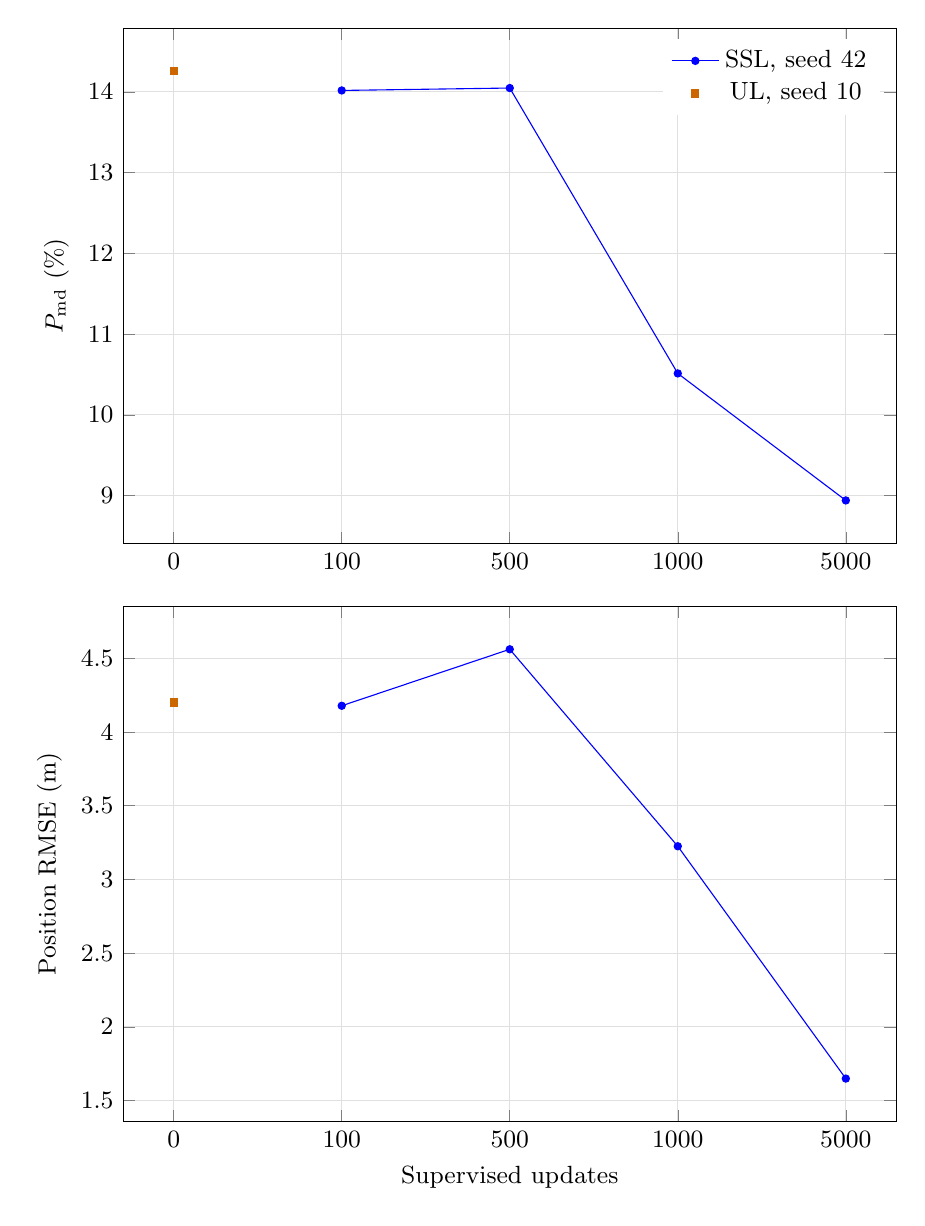
\begin{tikzpicture}
\begin{groupplot}[reportaxis,group style={group size=1 by 2,vertical sep=0.8cm}]
\nextgroupplot[xmin=-0.3,xmax=4.3,xtick={0,1,2,3,4},xticklabels={0,100,500,1000,5000},ylabel={$P_{\rm md}$ (\%)}]
\addplot[blue,mark=*] coordinates {(1,14.0169238) (2,14.0467894) (3,10.5126929) (4,8.93977103)};
\addplot[orange!80!black,only marks,mark=square*] coordinates {(0,14.2558487)};
\addlegendentry{SSL, seed 42}
\addlegendentry{UL, seed 10}
\nextgroupplot[xmin=-0.3,xmax=4.3,xtick={0,1,2,3,4},xticklabels={0,100,500,1000,5000},ylabel={Position RMSE (m)},xlabel={Supervised updates}]
\addplot[blue,mark=*] coordinates {(1,4.17837381) (2,4.56171608) (3,3.2250669) (4,1.64862156)};
\addplot[orange!80!black,only marks,mark=square*] coordinates {(0,4.19995403)};
\end{groupplot}\end{tikzpicture}
\caption{Fresh supervised-budget sweep at 85,000 total updates. The horizontal positions denote discrete tested allocations. Joint test thresholds and beams are selected before testing. The seed-10 UL point is an additional reference.}\label{fig:fraction-final}
\end{figure}\subsection{Sensing-SNR transfer}
Figure~\ref{fig:snr-final} evaluates frozen sweep models at five sensing SNRs. At low SNR, detection and localization deteriorate for every allocation. At 15 dB, the 5,000-supervised-update model attains the lowest PMD of the tested fresh models. The saved SNR arrays also report PFA, SER and detected-target RMSE at each frozen operating point. PFA can remain identical across sensing SNR for a given model because the absent-target null contains noise and the same calibration/test random seeds are reused. Communication SER changes little when only sensing SNR changes, although beam validation can choose another operating point.

The transfer test does not retrain the model at each noise level. It therefore measures the deployment of a fixed learned array with validation-based operating-point adjustment. Common random streams improve comparability between checkpoints but do not create multiple independent Monte Carlo replicates.
\begin{figure}[t]\centering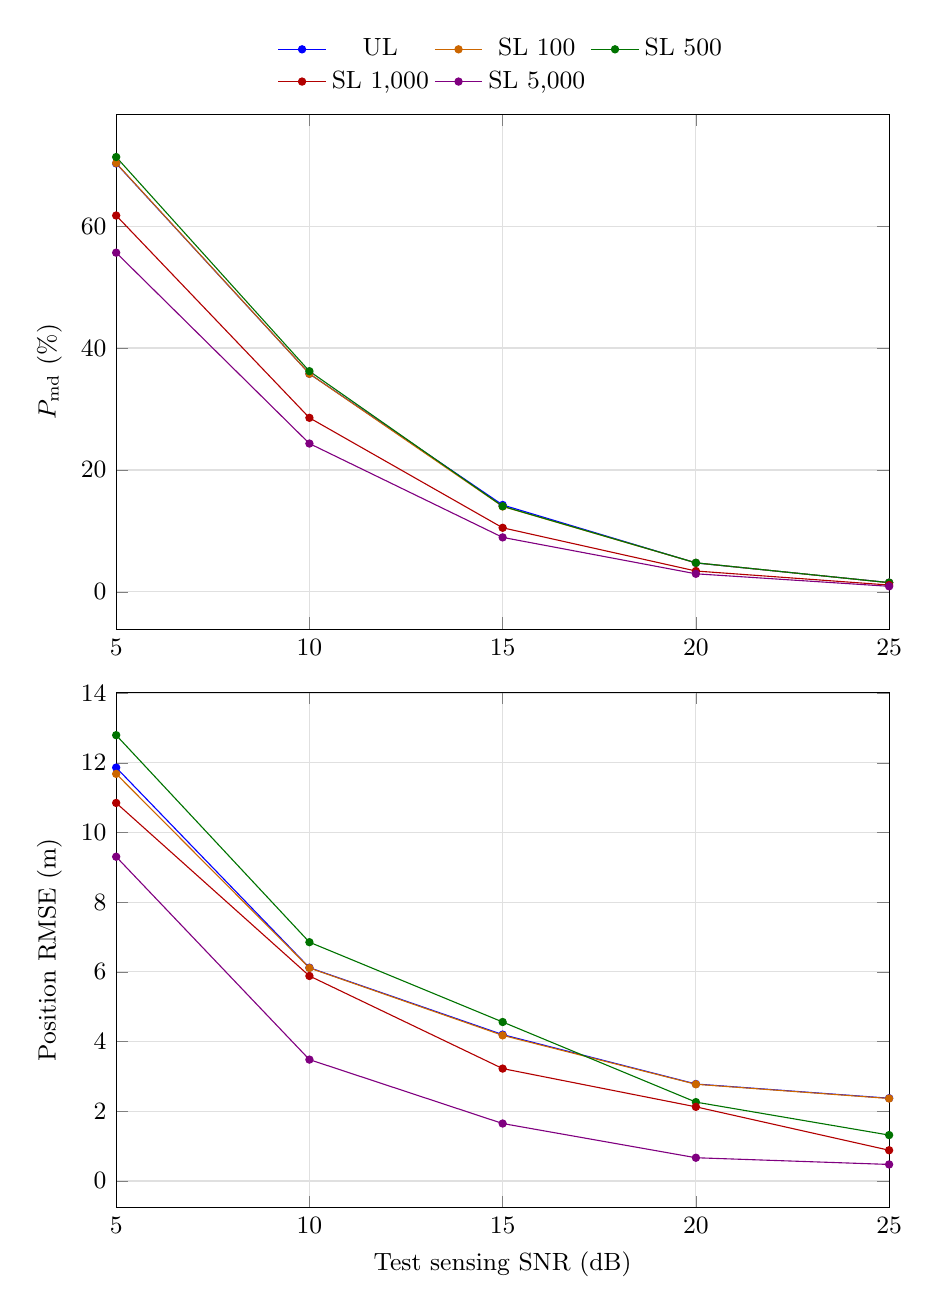
\begin{tikzpicture}
\begin{groupplot}[reportaxis,group style={group size=1 by 2,vertical sep=0.8cm}]
\nextgroupplot[xmin=5,xmax=25,xtick={5,10,15,20,25},ylabel={$P_{\rm md}$ (\%)},legend columns=3,legend style={at={(0.5,1.02)},anchor=south}]
\addplot[blue,mark=*] coordinates {(5,70.273768) (10,35.7789945) (15,14.2558487) (20,4.74863116) (25,1.52314584)};
\addlegendentry{UL}
\addplot[orange!80!black,mark=*] coordinates {(5,70.3235441) (10,35.7789945) (15,14.0169238) (20,4.75858636) (25,1.51319064)};
\addlegendentry{SL 100}
\addplot[green!45!black,mark=*] coordinates {(5,71.3290194) (10,36.197113) (15,14.0467894) (20,4.76854156) (25,1.51319064)};
\addlegendentry{SL 500}
\addplot[red!70!black,mark=*] coordinates {(5,61.7322051) (10,28.5515182) (15,10.5126929) (20,3.42458935) (25,1.12493778)};
\addlegendentry{SL 1,000}
\addplot[violet,mark=*] coordinates {(5,55.6396217) (10,24.3305127) (15,8.93977103) (20,2.96665007) (25,0.915878547)};
\addlegendentry{SL 5,000}
\nextgroupplot[xmin=5,xmax=25,xtick={5,10,15,20,25},ylabel={Position RMSE (m)},legend columns=3,legend style={at={(0.5,1.02)},anchor=south},xlabel={Test sensing SNR (dB)}]
\addplot[blue,mark=*] coordinates {(5,11.8627625) (10,6.1205411) (15,4.19995403) (20,2.78264046) (25,2.37476563)};
\addplot[orange!80!black,mark=*] coordinates {(5,11.6829433) (10,6.11269188) (15,4.17837381) (20,2.77544045) (25,2.36670232)};
\addplot[green!45!black,mark=*] coordinates {(5,12.7937355) (10,6.85207176) (15,4.56171608) (20,2.26306057) (25,1.3168453)};
\addplot[red!70!black,mark=*] coordinates {(5,10.848484) (10,5.88338709) (15,3.2250669) (20,2.12745285) (25,0.881628752)};
\addplot[violet,mark=*] coordinates {(5,9.30467892) (10,3.48290873) (15,1.64862156) (20,0.66678375) (25,0.474153727)};
\end{groupplot}\end{tikzpicture}
\caption{Sensing-SNR transfer of the completed sweep checkpoints. The legend gives supervised updates for SSL. UL uses seed 10 and SSL uses seed 42. Communication SNR remains 20 dB. A separate validation-selected operating point is frozen before each SNR test.}\label{fig:snr-final}
\end{figure}\subsection{Independent localization and error tails}
Table~\ref{tab:localization-final} reports the new 5,000-scene localization pool. It evaluates all present scenes over the broad training-sector distribution. The exact squared-position decomposition is
\begin{equation}
 \|\widehat{\mathbf p}-\mathbf p\|_2^2
 = (\widehat R-R)^2+2\widehat R R[1-\cos(\widehat\theta-\theta)].
 \label{eq:decomp}
\end{equation}
This permits direct accounting rather than an angular-error bound. A range outlier is defined by $|\widehat R-R|>2.5\Delta R$, with $\Delta R=c/(2S\Delta_f)\simeq4.88$ m. The top-1\% statistic is the share of total position MSE contributed by the 50 largest errors in the 5,000-scene pool.
\begin{table*}[t]\centering\small
\caption{Independent present-scene localization. Radial is the radial share of position MSE. Tail is the fraction of scenes exceeding the range-outlier threshold. Top 1\% is their largest-error MSE share.}\label{tab:localization-final}
\setlength{\tabcolsep}{3pt}
\begin{tabular}{lrrrrr}\toprule
Model & RMSE (m) & Median (m) & Radial (\%) & Tail (\%) & Top 1\% (\%)\\\midrule
UL, seed 10 & 14.689 & 0.767 & 97.1 & 3.38 & 73.0\\
SSL 100 & 14.383 & 0.757 & 97.0 & 3.34 & 73.2\\
SSL 500 & 15.481 & 0.768 & 97.6 & 3.20 & 76.2\\
SSL 1,000 & 14.044 & 0.525 & 98.1 & 2.70 & 80.4\\
SSL 5,000 & 13.532 & 0.402 & 98.5 & 2.34 & 82.4\\
Known array & 13.482 & 0.334 & 98.1 & 2.20 & 85.7\\
\bottomrule\end{tabular}
\end{table*}
For the fresh SSL checkpoints, unconditional RMSE remains 13.53--15.48 m while median errors range from 0.402 to 0.768 m. Radial error contributes 97.0--98.5\% of position MSE. Only 2.34--3.34\% of scenes exceed the range-outlier threshold, yet range-tail scenes contribute over 99\% of position MSE for those models. The top 1\% of errors contributes 73.2--82.4\% of total MSE. Even known hardware retains RMSE 13.482 m with median 0.334 m, showing that accurate array parameters alone do not remove the localization tail in this receiver.

The saved gain magnitudes support the historical weak-echo diagnosis. For SSL with 5,000 SL updates, the median gain is 0.074 among range-outlier scenes and 0.599 among other scenes. This is an observed association in one independent scene pool. It does not isolate the causal effect of gain or show that calibration cannot alter peak selection, because angular and range estimation share the joint map.
\section{Acquisition Ablations and Robustness}\label{sec:ablations}
\subsection{Controlled fixed-array ablations}
The corrected 50-run cohort gives final calibration error $0.1527\pm0.0237$ for weak acquisition, $0.1714\pm0.0117$ for random, and $0.1683\pm0.0241$ for fixed labels, where values are mean and 95\% halfwidth across five optimization seeds. The paired weak-minus-random calibration difference is $-0.0187\pm0.0259$, so its interval includes zero.

Table~\ref{tab:ablation-final} isolates the weak-subspace restriction, within-batch greedy update, and acquisition of new labels. Each row changes one component relative to the proposed method in the final row. D-optimal remains a comparator rather than the projection ablation because it changes the scalar objective as well. The calibration and central-sector legacy-frontier summaries correspond to the completed corrected cohort, preserving the evaluation protocol used when those controls were run.
\begin{table}[t]\centering\small
\caption{One-change acquisition ablations. All rows receive 2,200 updates. PMD uses the central-sector measured-frontier protocol. Entries are means with 95\% halfwidths across five seeds.}\label{tab:ablation-final}
\setlength{\tabcolsep}{3pt}
\begin{tabular}{lrrr}\toprule
Variant & Labels & $e_d$ & PMD (\%)\\\midrule
Full trace & 60 & $0.1527\pm0.0237$ & $8.729\pm0.080$\\
Greedy updates off & 60 & $0.1527\pm0.0237$ & $8.729\pm0.080$\\
New labels off & 10 & $0.1683\pm0.0241$ & $8.740\pm0.054$\\
Proposed method & 60 & $0.1527\pm0.0237$ & $8.729\pm0.080$\\
\bottomrule\end{tabular}
\end{table}
Central-sector PMD is 8.729\% for weak, 8.736\% for random and 8.740\% for fixed labels. The paired weak-minus-random difference is $-0.008\pm0.111$ percentage points. Thus the central test does not establish a detection advantage for acquisition. Uncertainty selection has mean calibration error 0.3017 and central PMD 10.453\%, with a wide PMD interval across seeds. Its historical selection of low-gain, near-broadside scenes helps explain why prediction uncertainty need not prioritize calibration information.

The independent evaluator was also run on every final active checkpoint, including nominal/known controls. Full per-checkpoint outputs are published in the completion CSV and JSON records. Their corrected operating-point values should be used for any later claim about deployment. Table~\ref{tab:ablation-final} is retained as the direct component-removal comparison from the cohort's original evaluation.

\subsection{Information-matrix diagnostic}
Weak, full-trace, D-optimal and both noRC variants have identical queried indices and saved round models across the corrected five seeds. We reconstruct candidate sets at rounds 1, 5 and 10 for all seeds. Every reconstructed weak batch matches the saved queries. Candidate label gains in each inspected round are nearly proportional to a shared matrix, with maximum relative residual $3.511\times10^{-9}$. The weak subspace has dimension one and weak/trace score correlation exceeds 0.999999999997.

For an approximate form $\Delta\F_i=c_i\mathbf M$, weak and full-trace scores are constant multiples of $c_i$. D-optimal gain is monotone in the same coefficient for positive-semidefinite increments. This explains the observed ranking agreement in the inspected rounds. A synthetic anisotropic matrix test makes weak and trace select different candidates, verifying that the implementations can distinguish directions. The experiment therefore provides no empirical separation of the weak-subspace and greedy components under these simulated conditions.

\subsection{Hardware and coverage results}
Table~\ref{tab:hardware-final} reproduces the completed hardware-study means. Its detection values use the common sensing sector $[-40,-20]^\circ$ under the legacy measured-frontier evaluation. Three optimization seeds are averaged within each of three independent arrays. The broad-coverage study contains the test sector within its support, whereas narrow training is evaluated in transfer.
\begin{table}[t]\centering\small
\caption{Hardware-study means over three independent arrays, each with three optimization seeds. Active variants use 60 unique labels and fixed uses 10.}\label{tab:hardware-final}
\setlength{\tabcolsep}{3pt}
\begin{tabular}{llrr}\toprule
Coverage & Method & $e_d$ & PMD (\%)\\\midrule
$\pm10^\circ$ & Guided & 0.1808 & 8.631\\
$\pm10^\circ$ & Random & 0.2034 & 9.994\\
$\pm10^\circ$ & Fixed & 0.1733 & 8.396\\
$\pm60^\circ$ & Guided & 0.1992 & 10.134\\
$\pm60^\circ$ & Random & 0.1617 & 9.034\\
$\pm60^\circ$ & Fixed & 0.1359 & 8.598\\
\bottomrule\end{tabular}
\end{table}
\begin{table}[t]\centering\small
\caption{Corrected independent-test hardware evaluation. Means and 95\% halfwidths use three array means, each averaging three optimization seeds. Differences are paired against random. Units are percent and percentage points (pp).}\label{tab:hardware-independent}
\setlength{\tabcolsep}{3pt}
\begin{tabular}{llrr}\toprule
Coverage & Method & PMD (\%) & Difference (pp)\\\midrule
$\pm10^\circ$ & Guided & $8.923\pm0.998$ & $-1.203\pm2.530$\\
$\pm10^\circ$ & Random & $10.127\pm1.549$ & $+0.000\pm0.000$\\
$\pm10^\circ$ & Fixed & $8.674\pm0.940$ & $-1.452\pm2.012$\\
$\pm60^\circ$ & Guided & $10.390\pm6.143$ & $+1.124\pm4.939$\\
$\pm60^\circ$ & Random & $9.266\pm1.245$ & $+0.000\pm0.000$\\
$\pm60^\circ$ & Fixed & $8.831\pm1.309$ & $-0.435\pm1.758$\\
\bottomrule\end{tabular}
\end{table}
The corrected frozen-point hardware tests in Table~\ref{tab:hardware-independent} give guided PMD 8.923\% under narrow coverage and 10.390\% under broad coverage. Random selection gives 10.127\% and 9.266\%, and fixed labels give 8.674\% and 8.831\%. Guided-minus-random differences are $-1.203\pm2.530$ and $+1.124\pm4.939$ percentage points. These intervals also include zero, so the independent test retains the absence of an established guided advantage. Operating-point selection is completed on validation data before these test values are observed.
Under narrow coverage, guided-minus-random calibration error is $-0.0226\pm0.0512$ and PMD differs by $-1.363\pm2.116$ percentage points. Under broad coverage the differences are $+0.0375\pm0.1914$ and $+1.100\pm5.220$ percentage points. All four intervals include zero. Fixed labels have the lowest mean calibration error and PMD in both coverages. Their narrow PMD difference to random narrowly excludes zero, but that comparison is exploratory among several tests over three arrays.

The four information comparators match weak selection in all 72 query comparisons across coverage, hardware and optimization seeds. Independent hardware and broad angular support therefore do not separate these criteria in this study. The shared scene pools and three arrays limit population-level conclusions. The negative result concerns the tested single-target, plug-in-information setting and budgets.

\subsection{Numerical checks and runtime}
The original model checks gave relative errors $1.57\times10^{-5}$ for channel agreement, $8.05\times10^{-6}$ for information-model means, and $1.15\times10^{-9}$ for automatic versus finite-difference Jacobians. Translation and scale transformations preserve the fixed-design mean up to modeled gain phase within approximately $1.5\times10^{-14}$. These checks validate local calculations without establishing global identifiability under bounded sectors.

The corrected pilot's acquisition computation averages about 24.0 s per weak run, 26.2 s per D-optimal run, and 0.003 s per random run. The original laptop CPU pilot required 711--736 s of training per run and belongs to a different execution environment. All full-budget fresh runs used a local RTX 4090 with PyTorch 2.5.1+cu121, and saved optimizer checkpoints every 1,000 updates. Table~\ref{tab:runtime-final} gives accumulated training time, excluding downtime, validation and test jobs.
\begin{table}[t]\centering\small
\caption{Measured fresh-run training time. All models receive 85,000 updates and batch size 3,000.}\label{tab:runtime-final}
\setlength{\tabcolsep}{3pt}
\begin{tabular}{rrr}\toprule
Supervised updates & Seed & Training (h)\\\midrule
0 & 10 & 22.94\\
100 & 42 & 19.96\\
500 & 42 & 13.74\\
1,000 & 42 & 13.41\\
5,000 & 42 & 12.02\\
\bottomrule\end{tabular}
\end{table}
\section{Discussion and Limitations}
The experiments answer two related questions with different evidence. The reproduction and fraction sweep assess the effect of spending optimization updates on position supervision. The acquisition experiments assess whether selecting additional fixed-scene position references helps beyond continued use of existing labels. The archived SSL result motivates sparse supervision, while the fresh sweep documents performance changes over four seed-42 allocations under independent operating-point testing. Neither observation by itself establishes the benefit of choosing which fixed scenes to label.

The acquisition controls support a qualified null finding. Information-based criteria agree exactly on labels under all tested hardware/coverage comparisons. Fixed-label continuation is competitive, and guided-minus-random hardware intervals include zero. The information criterion therefore lacks demonstrated incremental value over its simpler information comparators in this setting. The diagnostic gives a concrete reason for the criterion agreement without claiming that every possible ISAC configuration has proportional label gains.

Evaluation changes materially affect the reported numbers. The original sensing and joint-frontier routines remain relevant for matching the published code. Their threshold reuse, independently sorted interpolation, shared-range batches and large sample sizes differ from the independently calibrated frozen-point evaluation. We report both with explicit labels. Differences between those protocols are not training gains. Likewise, conditional detected-target RMSE and unconditional localization RMSE describe different populations and should be interpreted with their accompanying error-tail statistics.

Several limitations constrain the final claims. The fresh sweep has one optimization seed per supervised allocation, with an additional differently seeded UL reference. There are only three independent hardware draws and one shared scene pool per coverage. SNR transfer uses fixed checkpoints and validation adaptation, rather than independent retraining at each SNR. Test intervals condition on trained weights and calibrated thresholds and omit variation in training, scene-pool selection and calibration sets. A complete budget for reference measurements, tuning labels and acquisition computation has not been estimated. The active setup assumes repeatable interrogation of fixed scenes with valid reference positions.

The held-out localization data confirm a heavy range-error tail even with known array parameters. That supports reporting median error and exact MSE contributions alongside conditional RMSE. Because the receiver selects a peak in a joint angle--delay map, the observed radial dominance does not prove that the calibration estimate has no influence on range selection. Causal receiver modifications and broader scene/hardware distributions would require additional experiments.

\section{Conclusion}
We completed full-budget SL, UL and sequential SSL reproduction, a supervised-allocation sweep, repaired operating-point evaluation, controlled acquisition ablations, hardware/coverage repetitions, SNR transfer and independent localization analysis. The archived 1,000-SL/84,000-UL model approaches full-SL detection under the reproduction protocol. In the fresh seed-42 sweep, 5,000 supervised updates give lower independent-test misdetection than the smaller completed allocations and detected-target RMSE of 1.649 m. The active-calibration extension yields a reproducible null result under the tested model, with identical information-based queries, wide hardware intervals and competitive fixed-label continuation.

The principal limitations are sparse trained-model repetition, only three hardware draws, shared scene pools and incomplete unique-reference cost accounting. Future work should replicate supervised allocations across seeds, vary acquisition information geometry, and evaluate receiver changes targeting the measured localization tail. These conclusions follow the completed evidence while retaining the distinction between reproduction, independent testing and acquisition-budget experiments.
\appendices
\section{Nuisance Elimination and Training Loop}
Partition the information into hardware $u$ and nuisance $z$ blocks. The regularized effective information is
\begin{equation}
 \F_{u\mid z}=\mathbf I_{uu}-\mathbf I_{uz}(\mathbf I_{zz}+\epsilon\mathbf D)^{-1}\mathbf I_{zu},
\end{equation}
where $\epsilon\mathbf D$ is a trace-scaled ridge. The unlabeled calculation eliminates angle, range and complex gain. The labeled calculation eliminates only complex gain, and the soft sector precision enters only the unlabeled angle block. Derivatives condition on the transmitted beam.

The loop initializes at nominal spacing, trains SL then UL, estimates candidate geometry/gain, computes information gains, selects a batch, reveals positions, and repeats training/evaluation. Figure~\ref{fig:workflow} shows the cycle. Validation metrics do not enter optimization gradients.
\begin{figure}[!htb]\centering
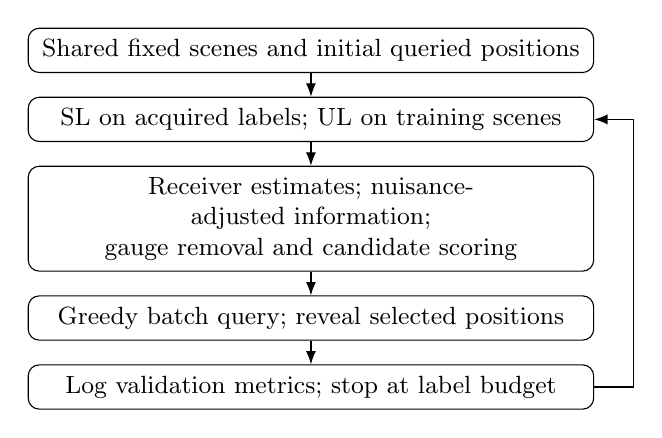
\begin{tikzpicture}[>=Latex,box/.style={draw,rounded corners,align=center,text width=6.9cm,font=\small,inner sep=4pt},node distance=3mm]
\node[box] (pool) {Shared fixed scenes and initial queried positions};
\node[box,below=of pool] (train) {SL on acquired labels; UL on training scenes};
\node[box,below=of train] (score) {Receiver estimates; nuisance-adjusted information;\\gauge removal and candidate scoring};
\node[box,below=of score] (query) {Greedy batch query; reveal selected positions};
\node[box,below=of query] (eval) {Log validation metrics; stop at label budget};
\draw[->] (pool)--(train);
\draw[->] (train)--(score);
\draw[->] (score)--(query);
\draw[->] (query)--(eval);
\draw[->] (eval.east)--++(.5cm,0)|-(train.east);
\end{tikzpicture}
\caption{Implemented acquisition and training cycle. Fresh measurements interrogate fixed scenes. The return path applies while the label budget remains.}\label{fig:workflow}
\end{figure}\section{Reference Tables}
\begin{table}[t]\centering\small
\caption{Completed experiment configurations. The active preset executes on CUDA when available.}\label{tab:settings-final}
\setlength{\tabcolsep}{3pt}
\begin{tabular}{lrrr}\toprule
Setting & Reproduction & Active & Fresh sweep\\\midrule
Total updates & 85,000 & 2,200 & 85,000\\
Batch size & 3,000 & 64 & 3,000\\
SL/UL rate & $(4/5)10^{-7}$ & $(4/5)10^{-6}$ & $(4/5)10^{-7}$\\
Train scenes & Online & 2,000 fixed & Online\\
Initial/final labels & Online & 10/60 & Online\\
Test frames/beam & 1,200,000 & 9,984 legacy & 20,000 final\\
Beam grid & $8\times8$ & $4\times4$ & $4\times4$\\
\bottomrule\end{tabular}
\end{table}
\begin{table*}[t]\centering\small
\caption{The 12 reviewed works. Settings and results are as reported by their authors.}\label{tab:related}
\begin{tabularx}{\textwidth}{>{\raggedright\arraybackslash}p{3.2cm}YYp{3.1cm}}\toprule
Work & Setting & Reported result & Role in our study\\\midrule
Model-based DL~\cite{mbdl} & Review of structured learning & Taxonomy of model-based designs & Learning framework\\
Model-driven ISAC~\cite{icc} & $K=16$, one target, spacing errors ($\sigma=\lambda/30$) & 2,500 complex parameters stay near full-complexity performance; a 5,000-parameter network degrades & Preceding architecture\\
Semi-supervised ISAC~\cite{ssl} & $K=64$, $S=256$, 85,000 updates & About 1.2\% supervised updates match full SL; degrades below about 1\% & Reproduction baseline\\
Multi-target ISAC~\cite{multi} & $K=64$, up to 5 targets, 15,000 updates & 64 learned spacings approach known-impairment detection with $720\times$ fewer parameters than a dictionary & Calibration scope\\
Gain--phase calibration~\cite{gain} & $K=64$, unsupervised, $10^4$ updates & Close to known-impairment sensing & Calibration scope\\
Differentiable MUSIC~\cite{music} & Direction of arrival, location and gain errors & More accurate than classical MUSIC & Calibration scope\\
Unsupervised multi-target~\cite{multiul} & Coherent signals, no labels & Preprint; alternative sensing objectives & Subsequent work\\
Array self-calibration~\cite{weiss} & Maximum likelihood, sources at unknown directions & Joint geometry and direction estimates & Nuisance coupling, gauge\\
Statistical acquisition~\cite{cohn} & Variance reduction for regression & Closed-form query criteria & Selection rationale\\
Core-set / BADGE~\cite{coreset,badge} & Feature-space coverage; gradient embeddings & Gains over random and uncertainty sampling on image benchmarks & Diversity comparator\\
BAIT~\cite{bait} & Last-layer Fisher, trace criterion & Matches or beats BADGE and Core-set on classification and regression & Information comparator\\\bottomrule
\end{tabularx}
\end{table*}
\section{Reproducibility and Artifact Access}
The final repository is \url{https://github.com/muneefo/DL_FINAL_REPORT}. It includes source, generated tables/figures, raw arrays, checkpoints and run logs. Git LFS stores the large ZIP archives. The imported baseline is \url{https://github.com/josemateosramos/SSLISAC}, associated with~\cite{ssl}. The team's earlier extension repository is \url{https://github.com/andrewliang-uwcs/867-deep-learning}. The original archive's precise upstream commit was not recorded, and should not be inferred from a later repository head. Original license and source attribution are retained.

The top-level \texttt{lib/}, \texttt{methods/} and \texttt{results/} preserve the reproduction workspace. Extended scripts live in \texttt{final-report-work/}. The completed cohorts are named \texttt{final\_stage\_20261108-142922}, \texttt{hardware\_study\_20261108-160301} and \texttt{course\_completion\_20261109-133839}. The completion state records successful jobs and final status. Hardware manifests include source hashes and environment captures. Fresh fraction checkpoints include learning rates, seeds, allocations, timing, model/optimizer state and CPU/CUDA random states.

The command \texttt{python} \path{reports/make_submission_tables.py} mechanically regenerates the saved main and ablation evidence. \texttt{plot\_completion\_results.py} regenerates the sweep and SNR graphics. \texttt{build\_final\_report.py} builds this report from manuscript components and saved results. Its bibliography is \texttt{refs.bib}, compiled with IEEEtran style. Full retraining is expensive and separate from table generation. The release contains the completed raw results so graders can verify values without retraining.

\section{Contribution and Assistance Disclosure}
The original team statement assigns Muneef leadership of baseline reproduction, mathematical methodology, extension planning and experimental analysis. Andrew contributed to proposal writing, related-work synthesis and integration. Mohammad contributed to the evaluation plan. Andrew and Mohammad also contributed to results discussion, and all members contributed to the midterm report. The team must verify the final individual allocation against its actual work and earlier repository history before submission. This imported repository snapshot does not reconstruct earlier author commits.

AI assistance supported code implementation, experiment orchestration, evaluation auditing, diagnostic reasoning, numerical summaries, plotting and manuscript drafting. This includes assistance beyond grammar correction or boilerplate. The course specification restricts AI generation of the core methodological contribution or analysis. The team must accurately disclose the scope, establish ownership and understanding of the scientific work, and clarify acceptability with the instructor. The present draft does not certify that those human review and policy checks have been completed.

\section{Data Use}
The experiments use synthetic single-target sensing and communication scenes generated by the supplied physical model. No human-subject, medical or restricted external dataset is used in the reported experiments. Scene seeds and checkpoint metadata identify the generated pools. Public release of synthetic artifacts is governed by the retained source license and the team's attribution obligations.

\clearpage\raggedbottom\bibliographystyle{IEEEtran}\bibliography{refs}
\end{document}
